%\begin{figure*}[t]
%    \centering
%    \begin{tabular}{c c c}
%        \raisebox{1cm}{\rotatebox{90}{\parbox{3cm}{\centering Jasper Ridge}}} &
%        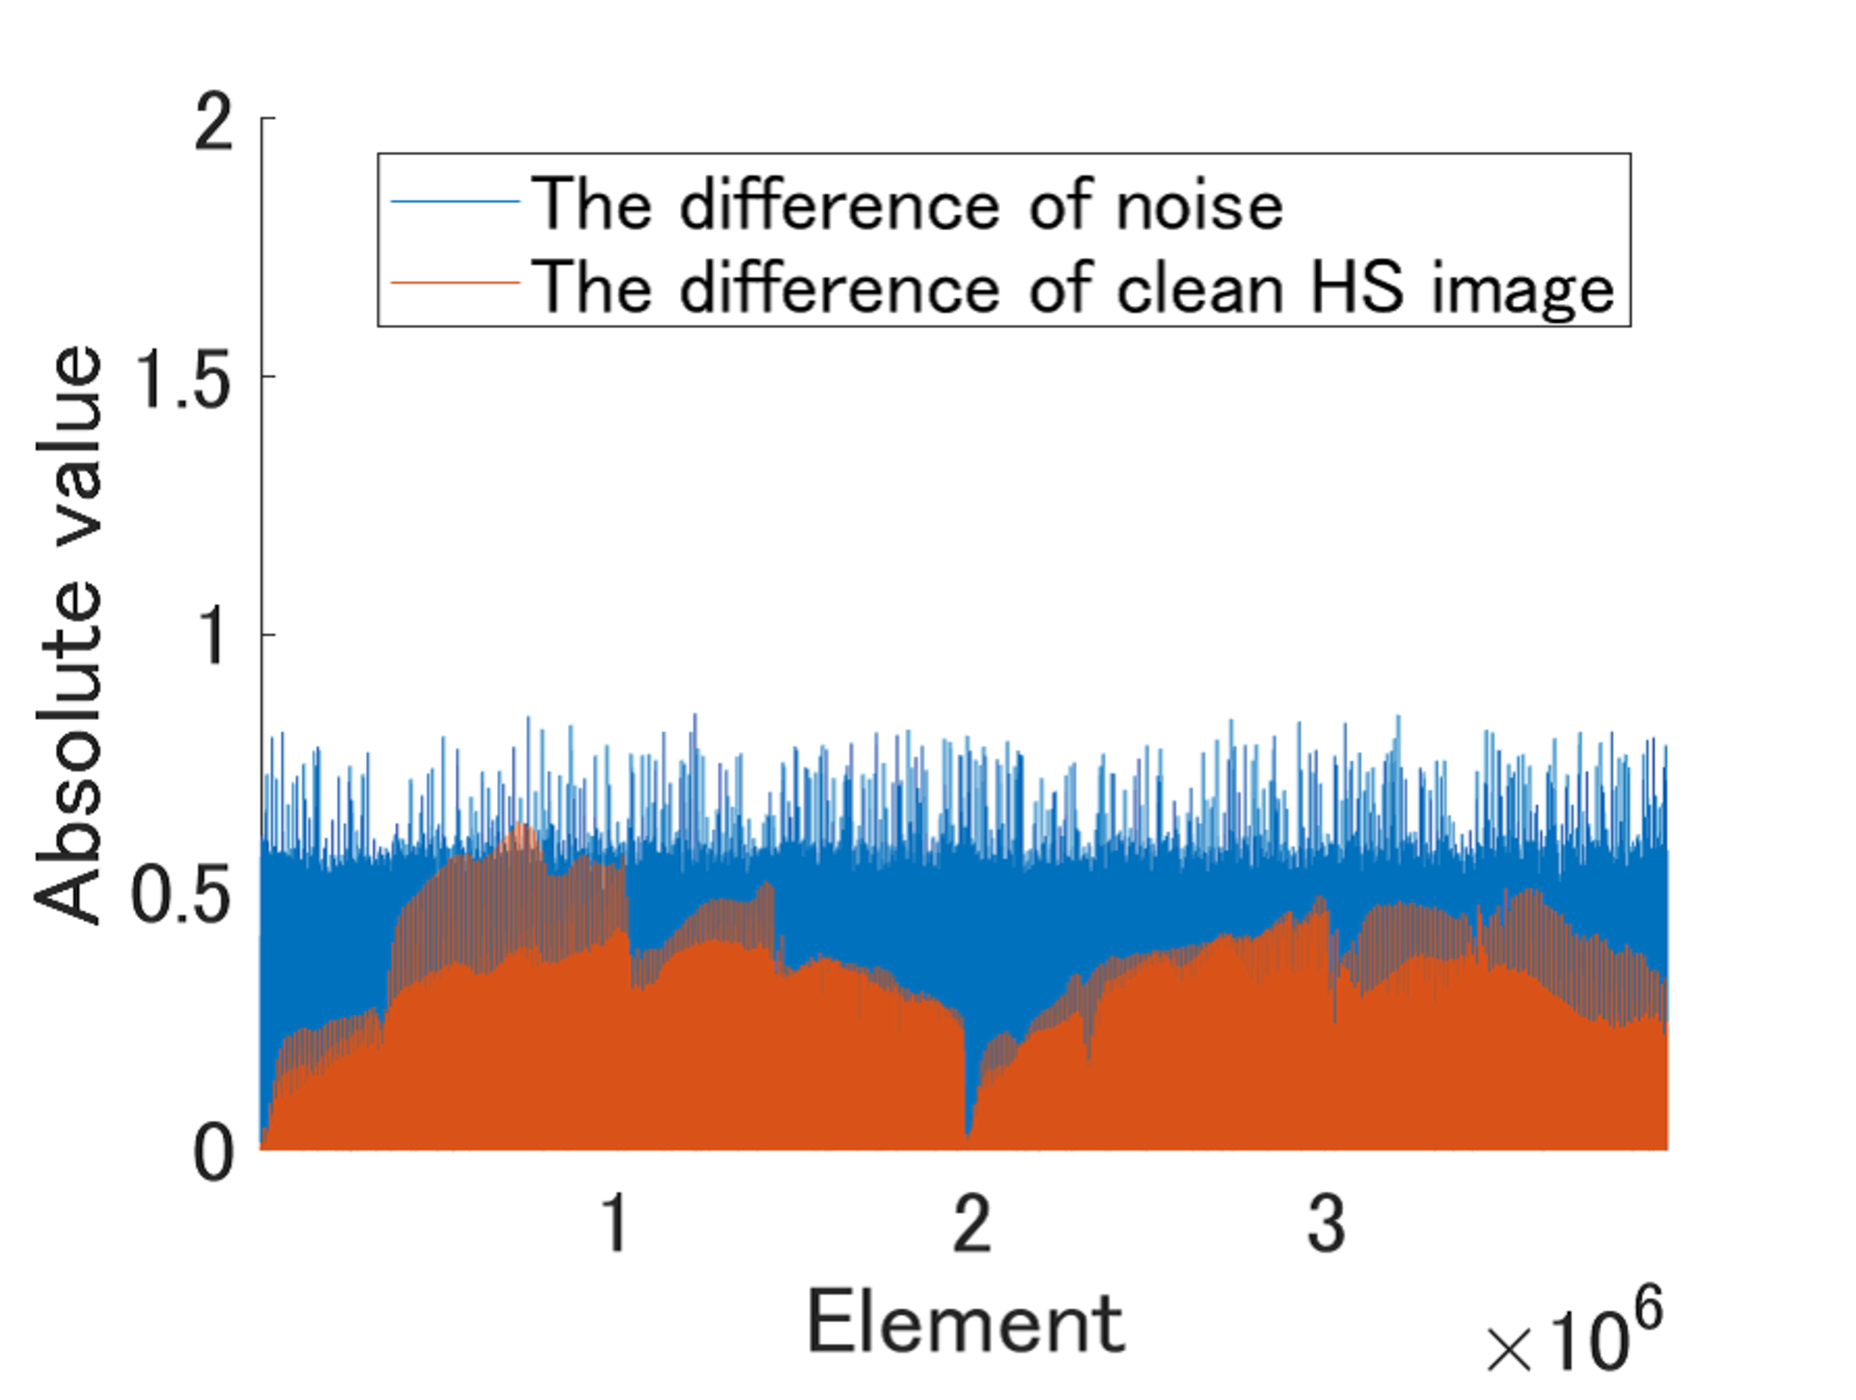
\includegraphics[width=0.4\textwidth]{./fig_supplement/compare_sparsity/JasperRidge_first_order_differences.eps} &
%        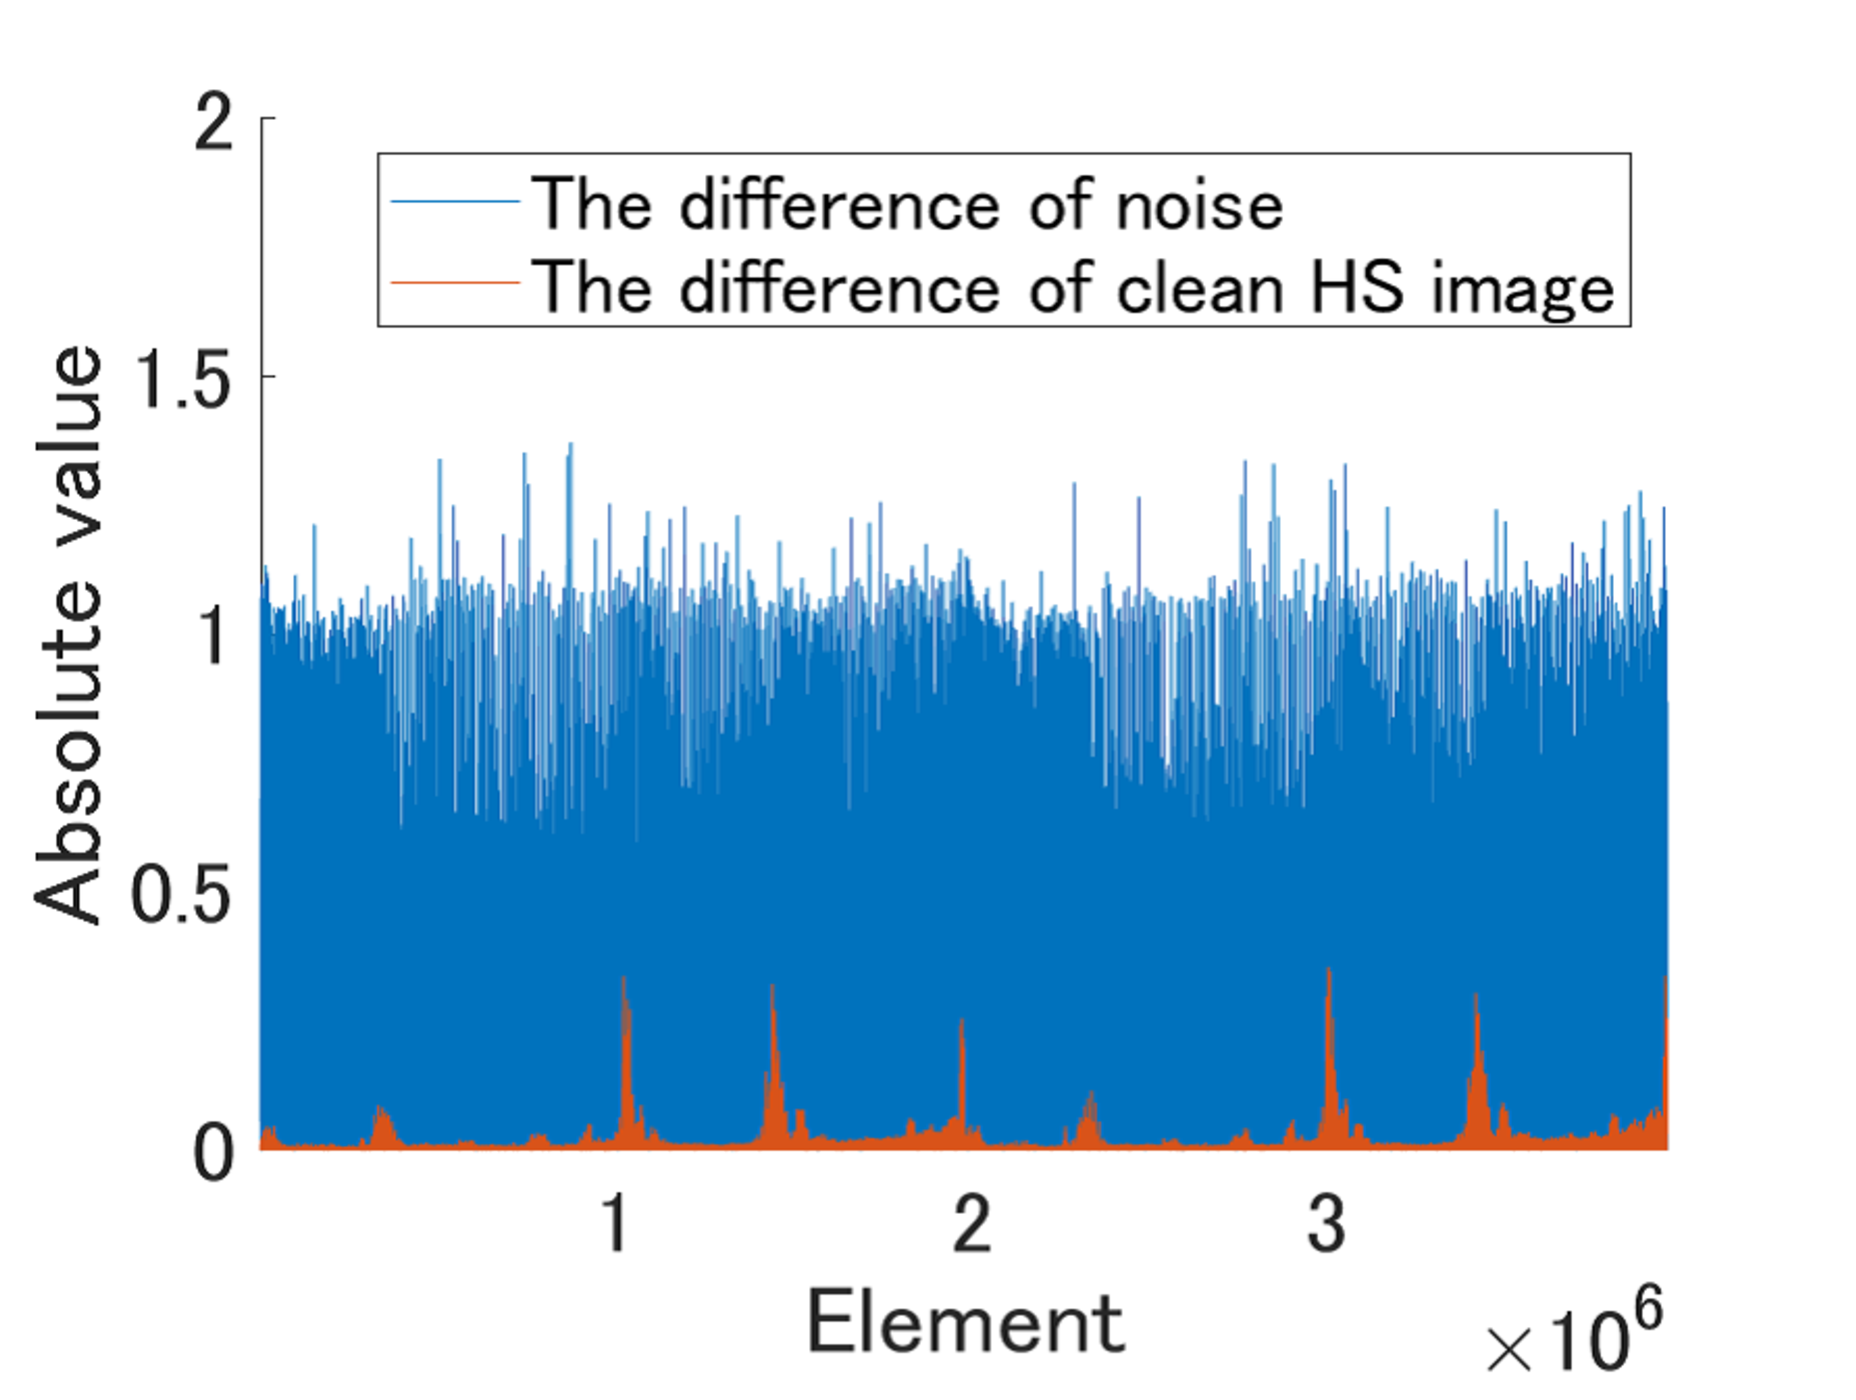
\includegraphics[width=0.4\textwidth]{./fig_supplement/compare_sparsity/JasperRidge_second_order_differences.eps} \\
%        
%        \raisebox{1cm}{\rotatebox{90}{\parbox{3cm}{\centering Pavia University}}} &
%        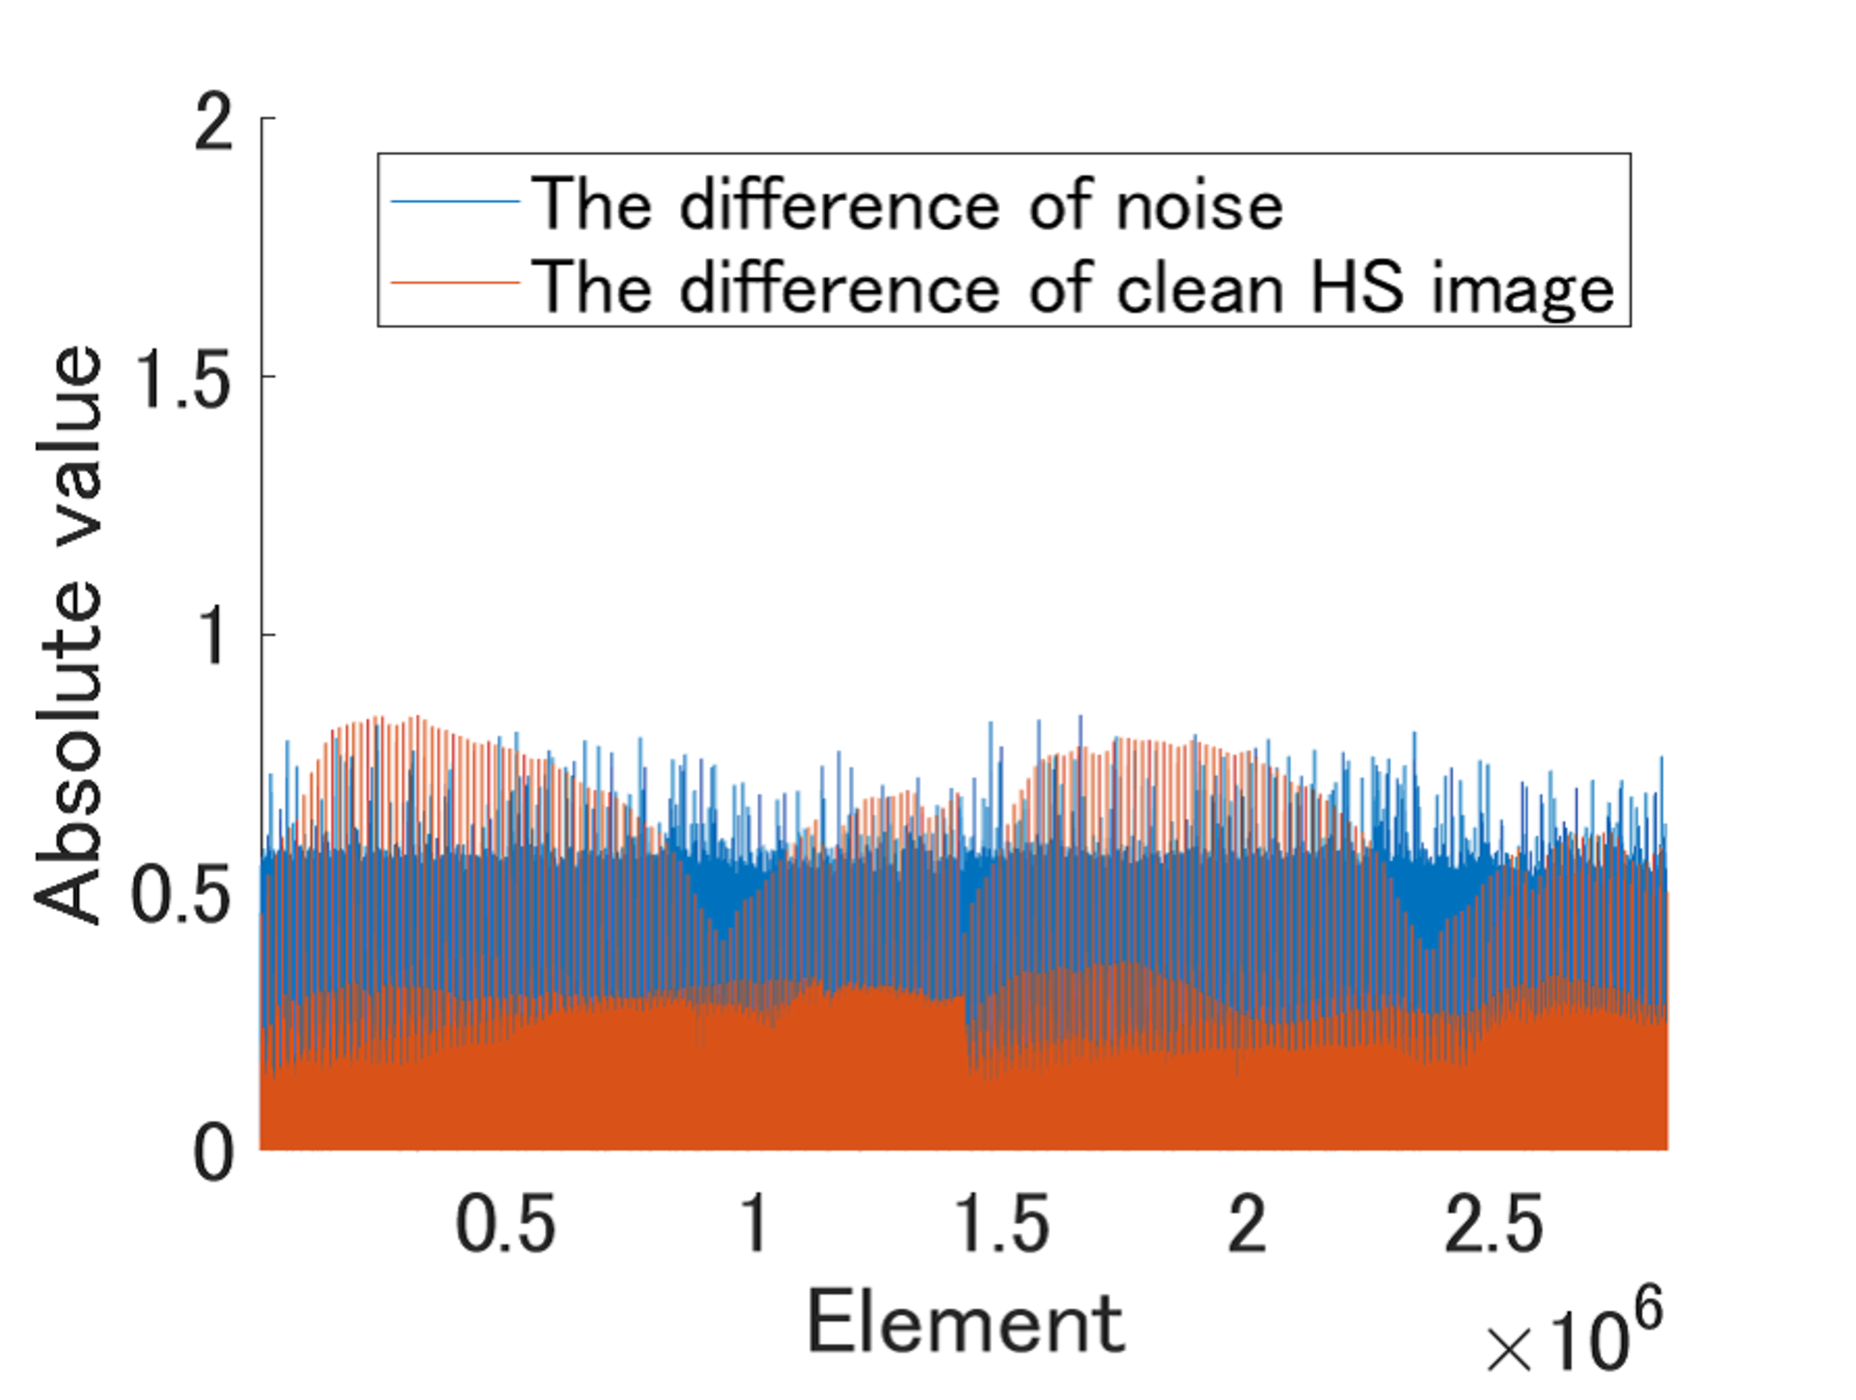
\includegraphics[width=0.4\textwidth]{./fig_supplement/compare_sparsity/PaviaU120_first_order_differences.eps} &
%        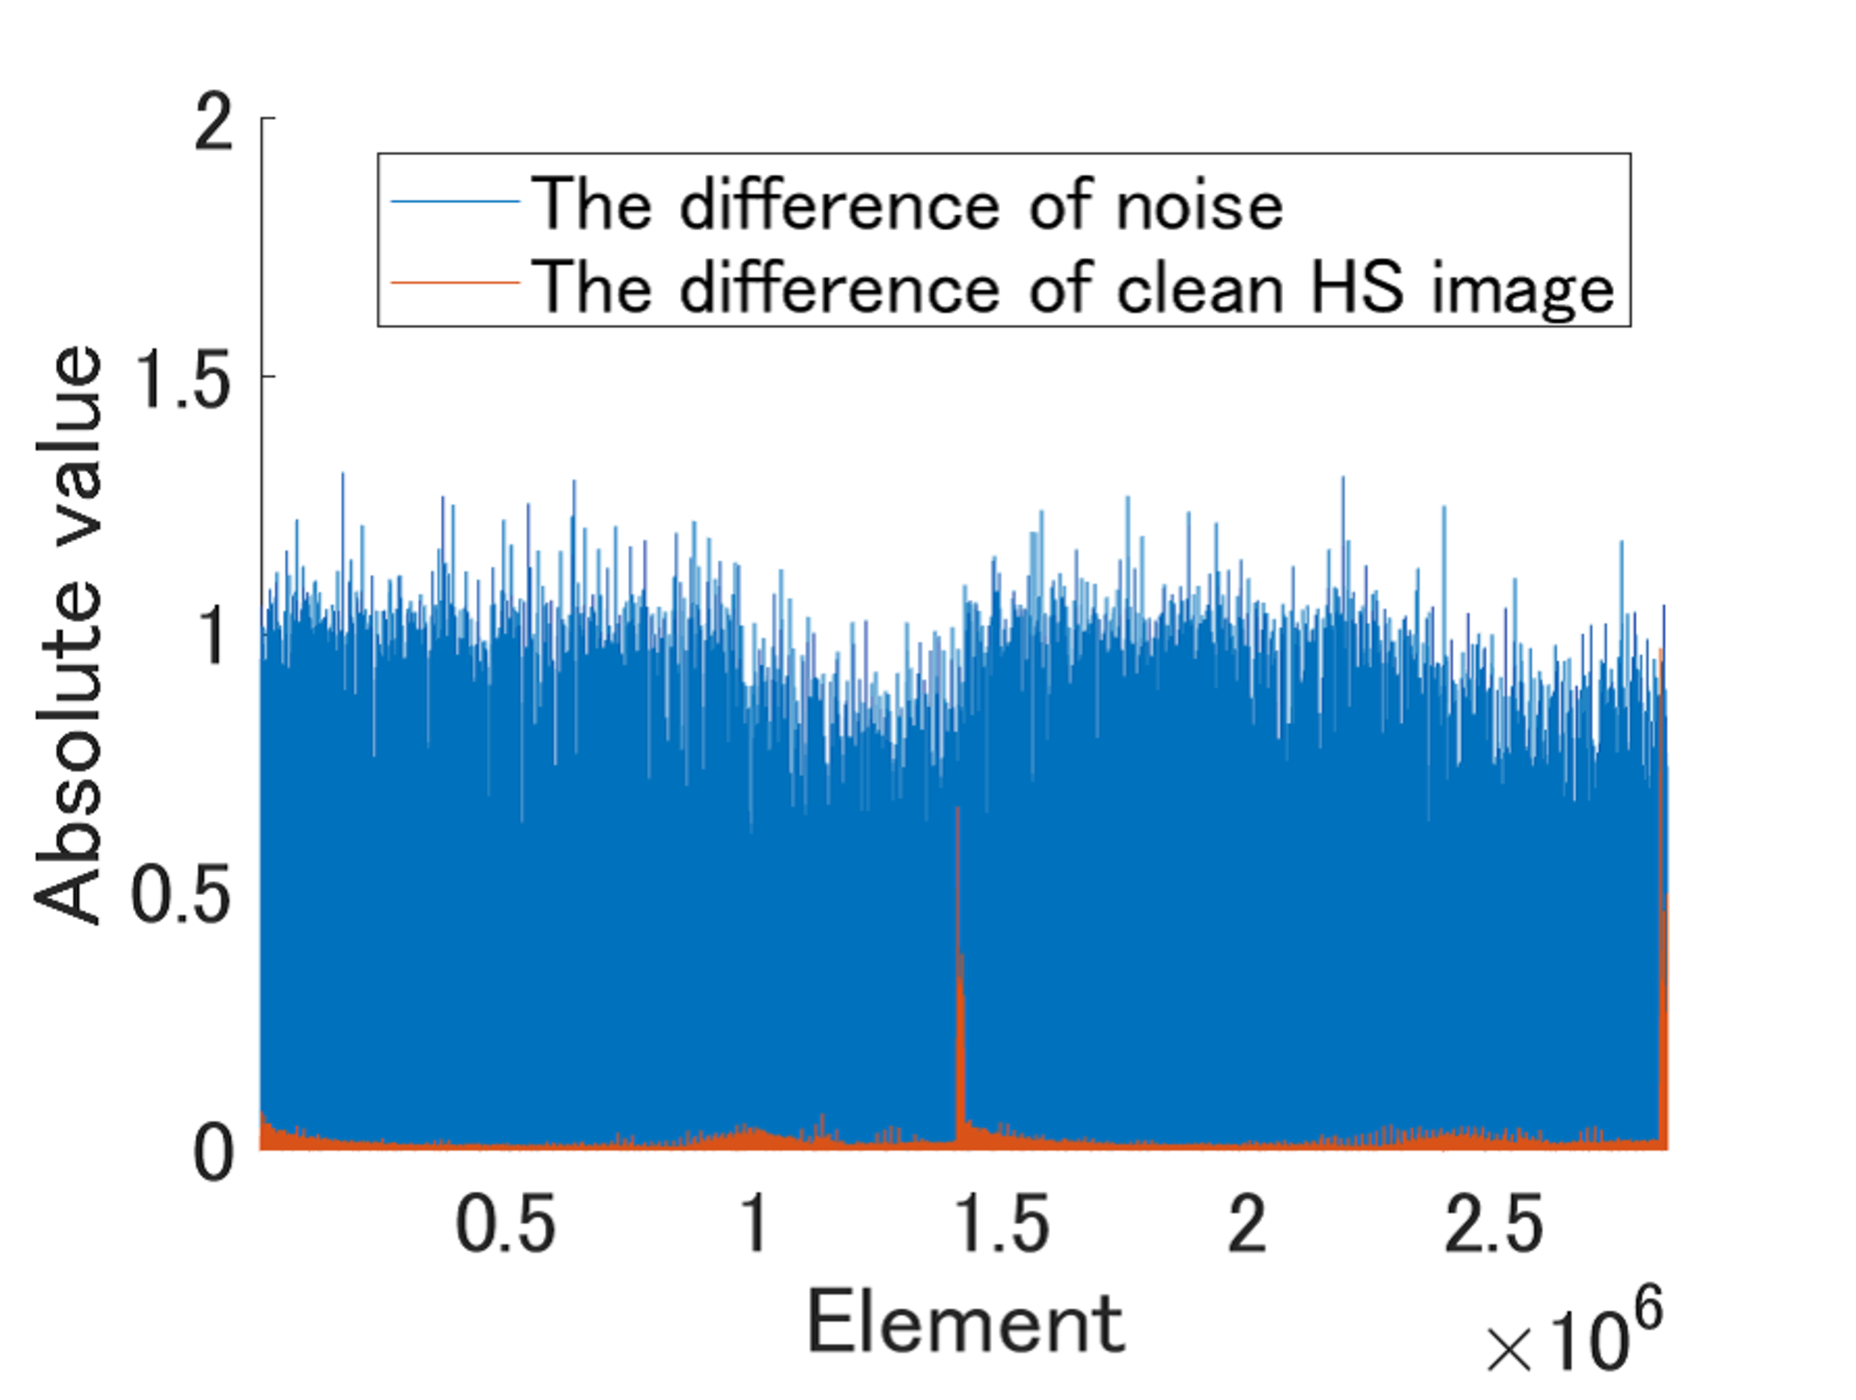
\includegraphics[width=0.4\textwidth]{./fig_supplement/compare_sparsity/PaviaU120_second_order_differences.eps} \\
%        
%        \raisebox{1cm}{\rotatebox{90}{\parbox{3cm}{\centering Beltsville}}} &
%        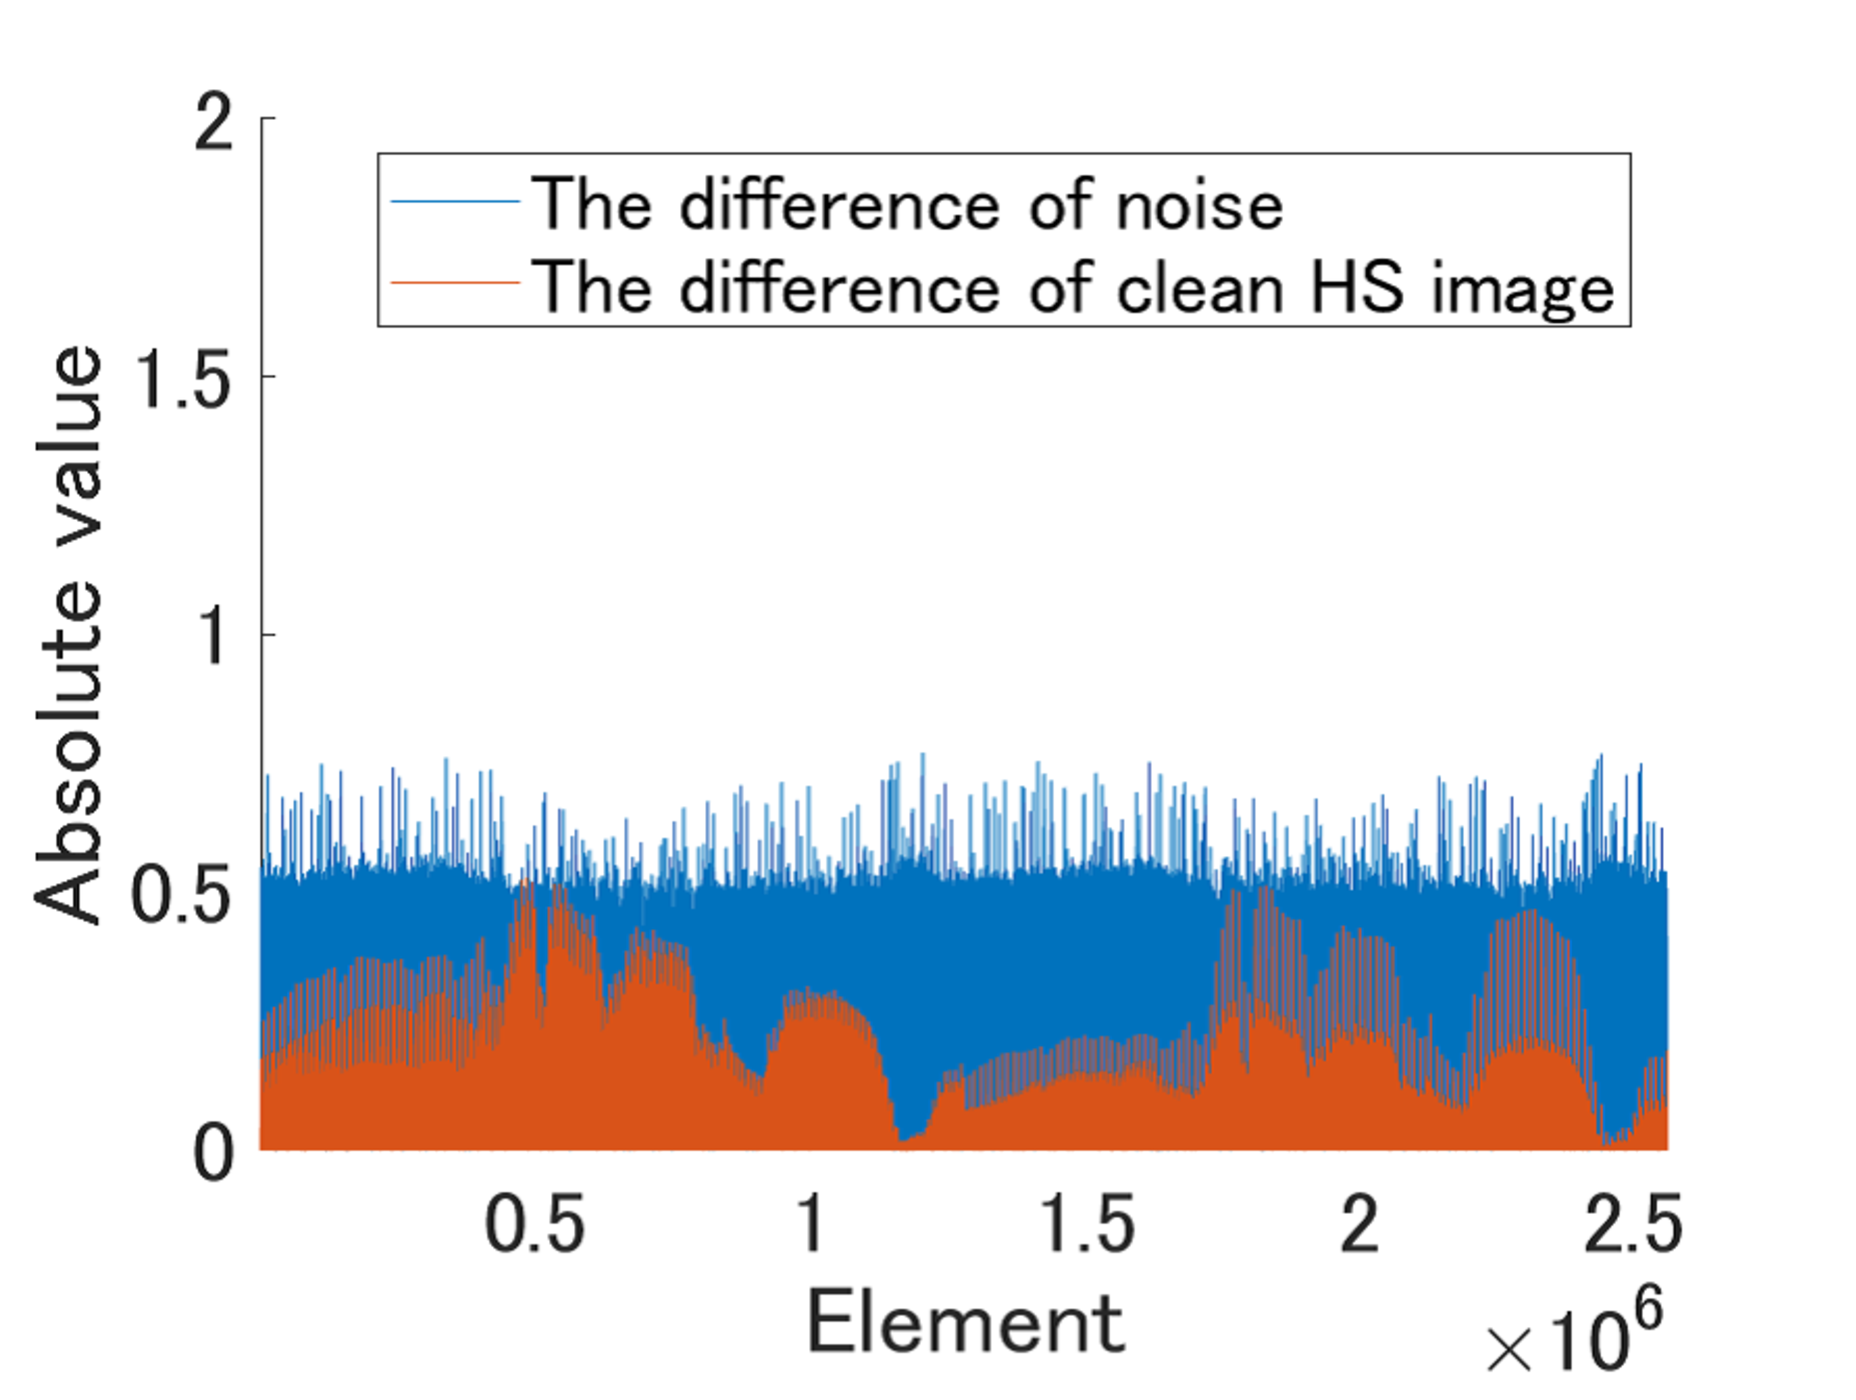
\includegraphics[width=0.4\textwidth]{./fig_supplement/compare_sparsity/Beltsville_first_order_differences.eps} &
%        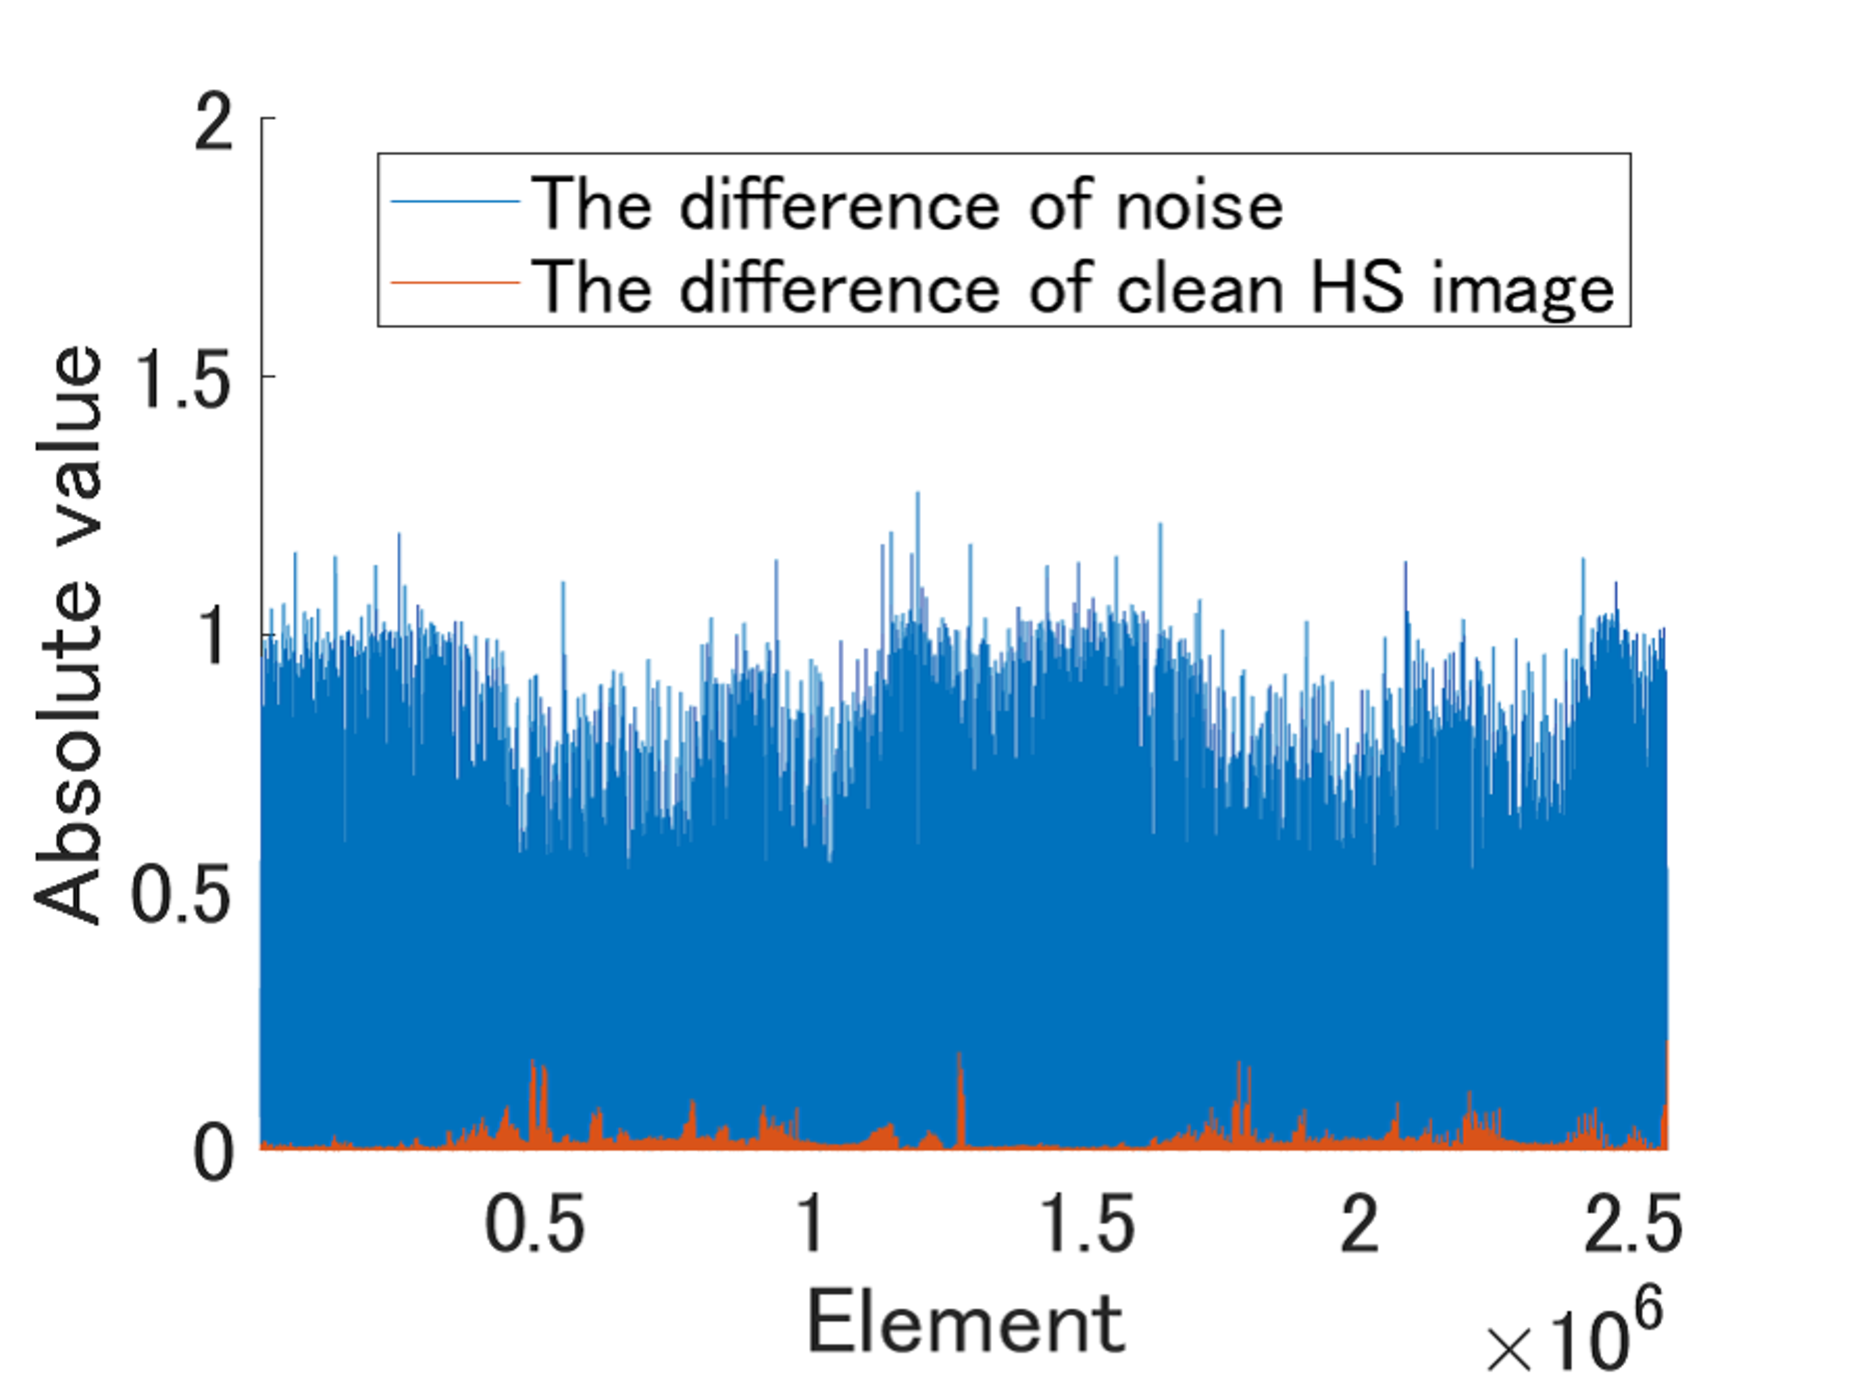
\includegraphics[width=0.4\textwidth]{./fig_supplement/compare_sparsity/Beltsville_second_order_differences.eps} \\
%    \end{tabular}
%    \caption{The absolute values of first-order (left) and second-order (right) differences for Jasper Ridge, Pavia University, and Beltsville}
%    
%    \label{fig:comparison_sparsity}
%\end{figure*}

\begin{figure*}[t]
	\begin{center}
		\makebox[0pt][r]{\raisebox{-6mm}{\rotatebox{90}{\shortstack{First-order\\ differences}}} \hspace{2mm}}%
		\begin{minipage}{0.320\hsize}
			\centerline{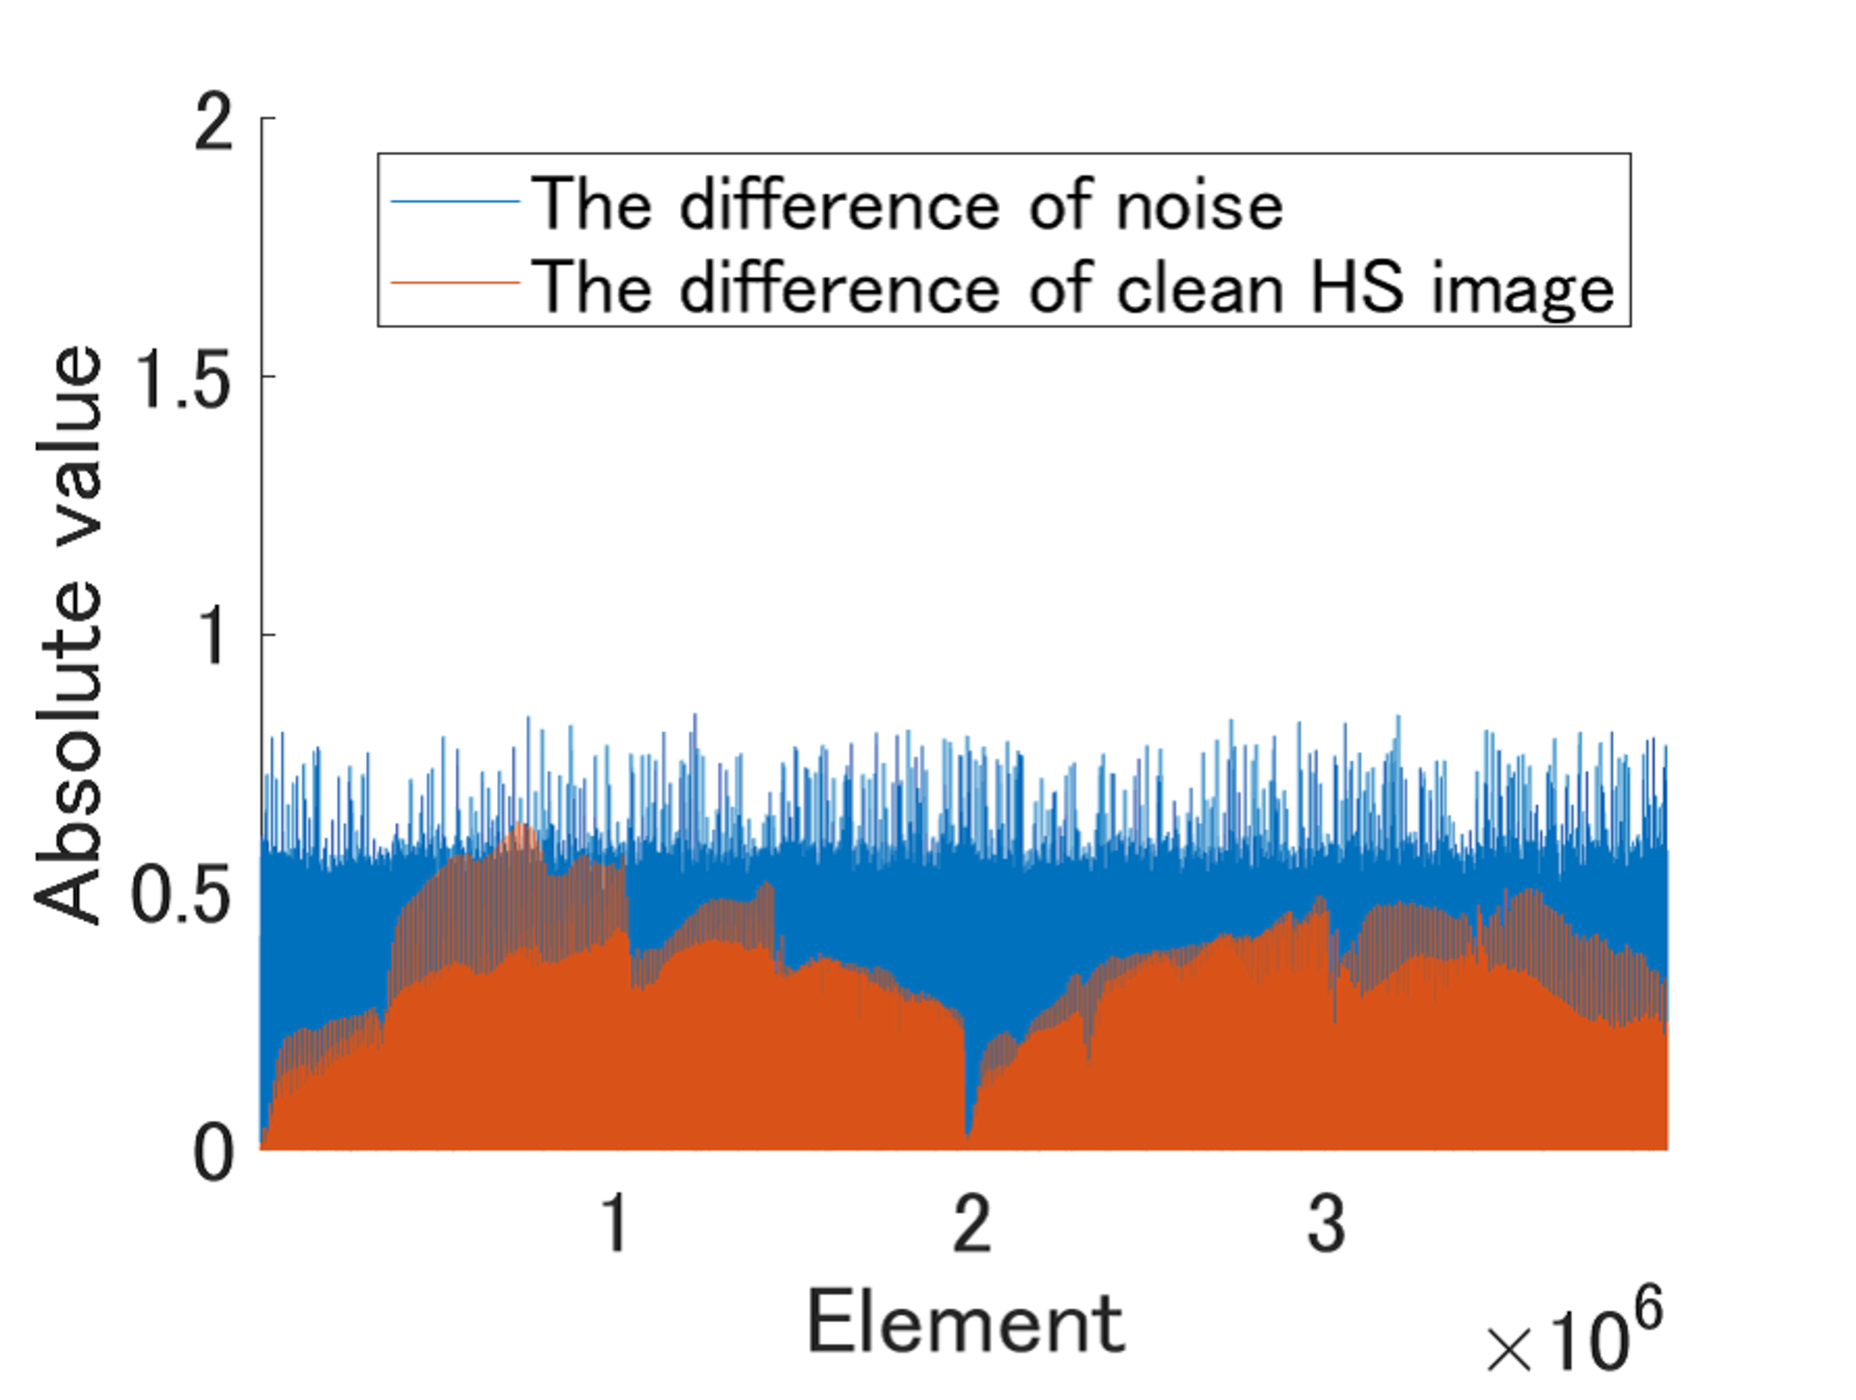
\includegraphics[width=\hsize]{./fig_supplement/compare_sparsity/JasperRidge_first_order_differences.eps}}
		\end{minipage}
		\begin{minipage}{0.320\hsize}
			\centerline{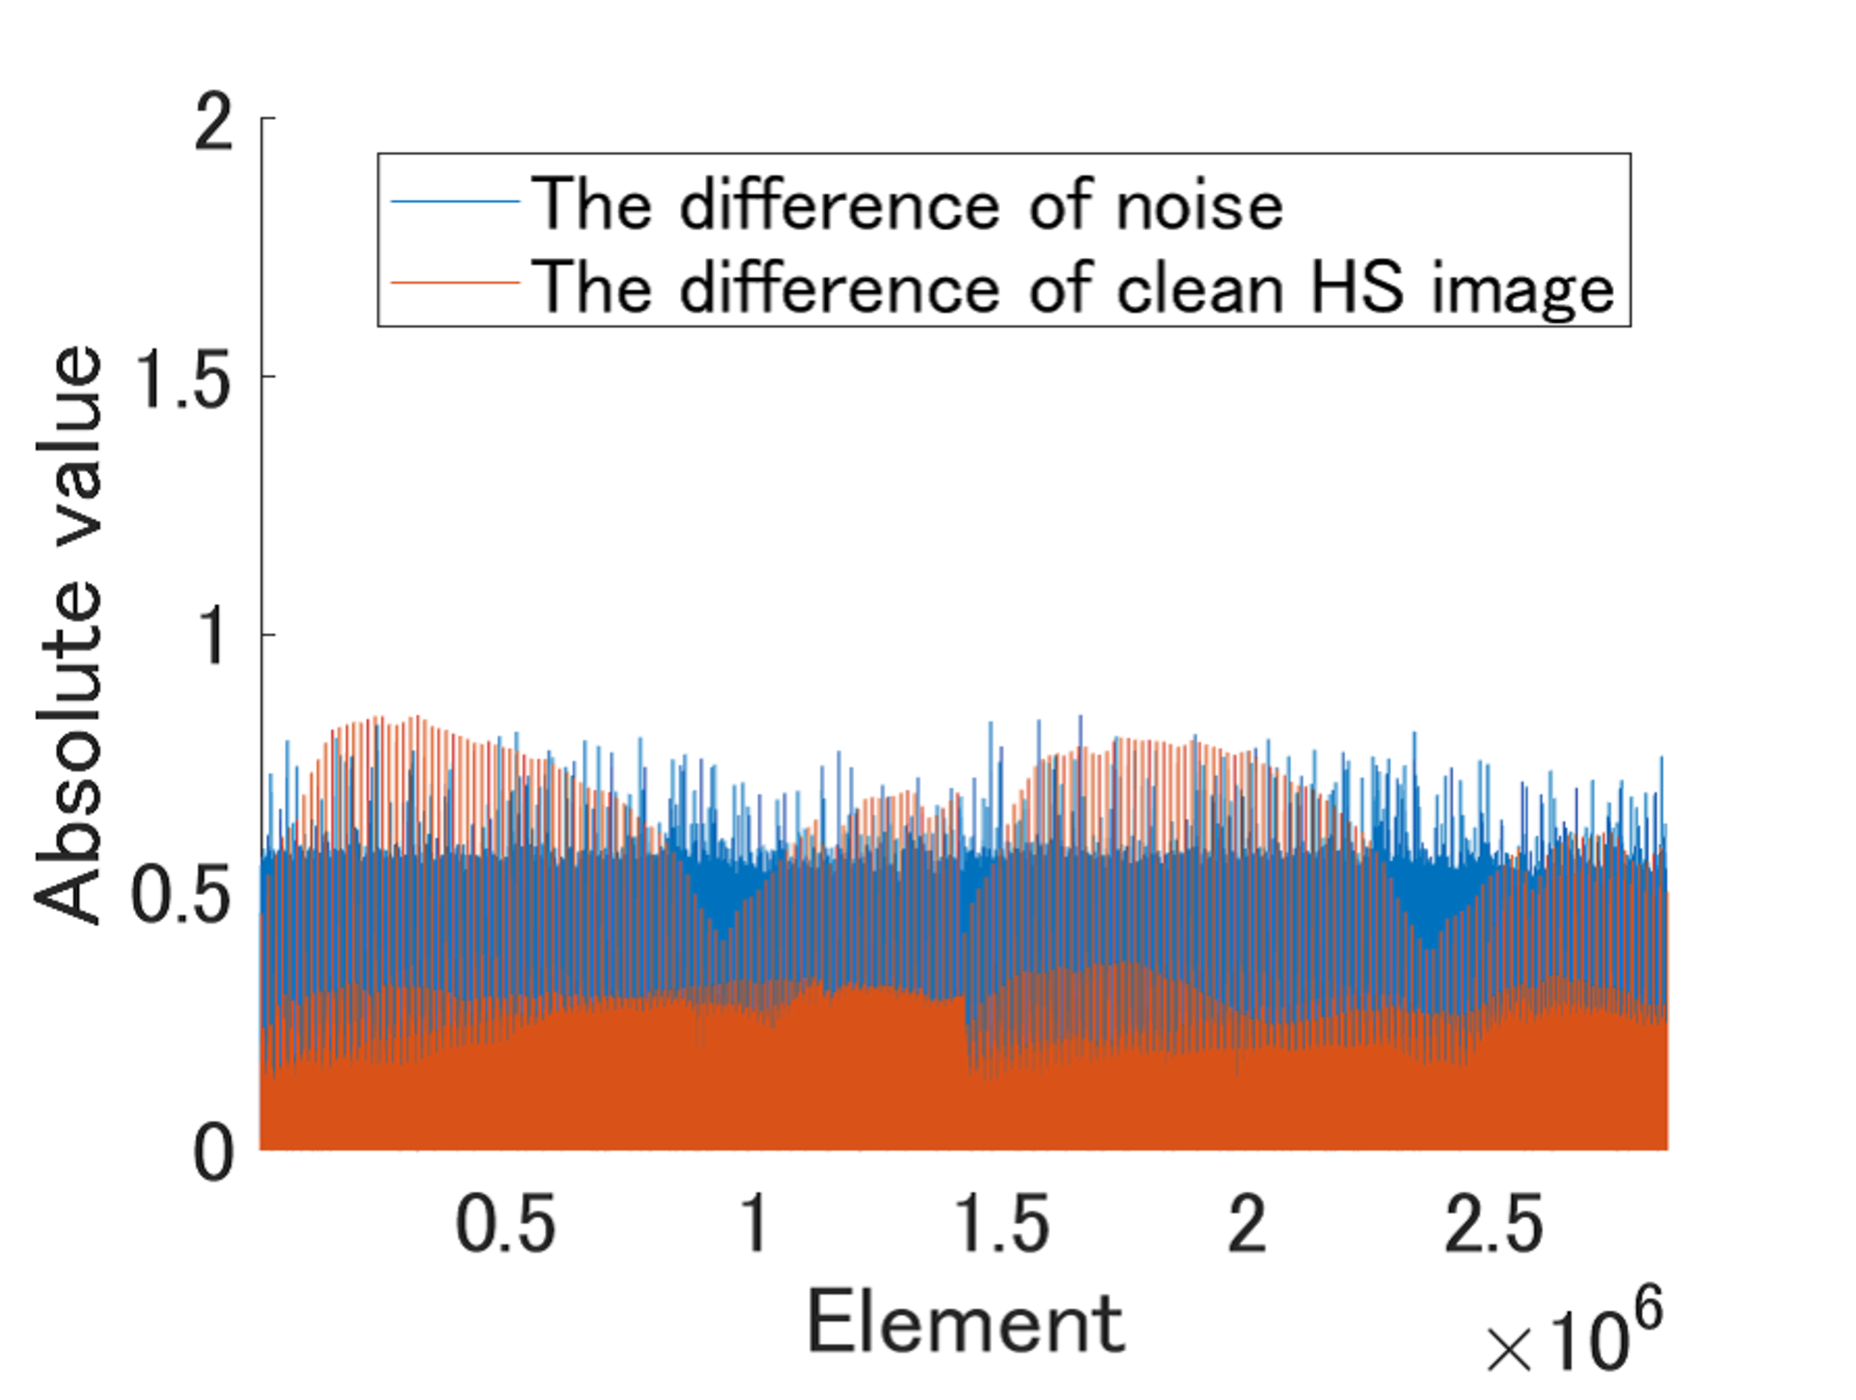
\includegraphics[width=\hsize]{./fig_supplement/compare_sparsity/PaviaU120_first_order_differences.eps}}
		\end{minipage}
		\begin{minipage}{0.320\hsize}
			\centerline{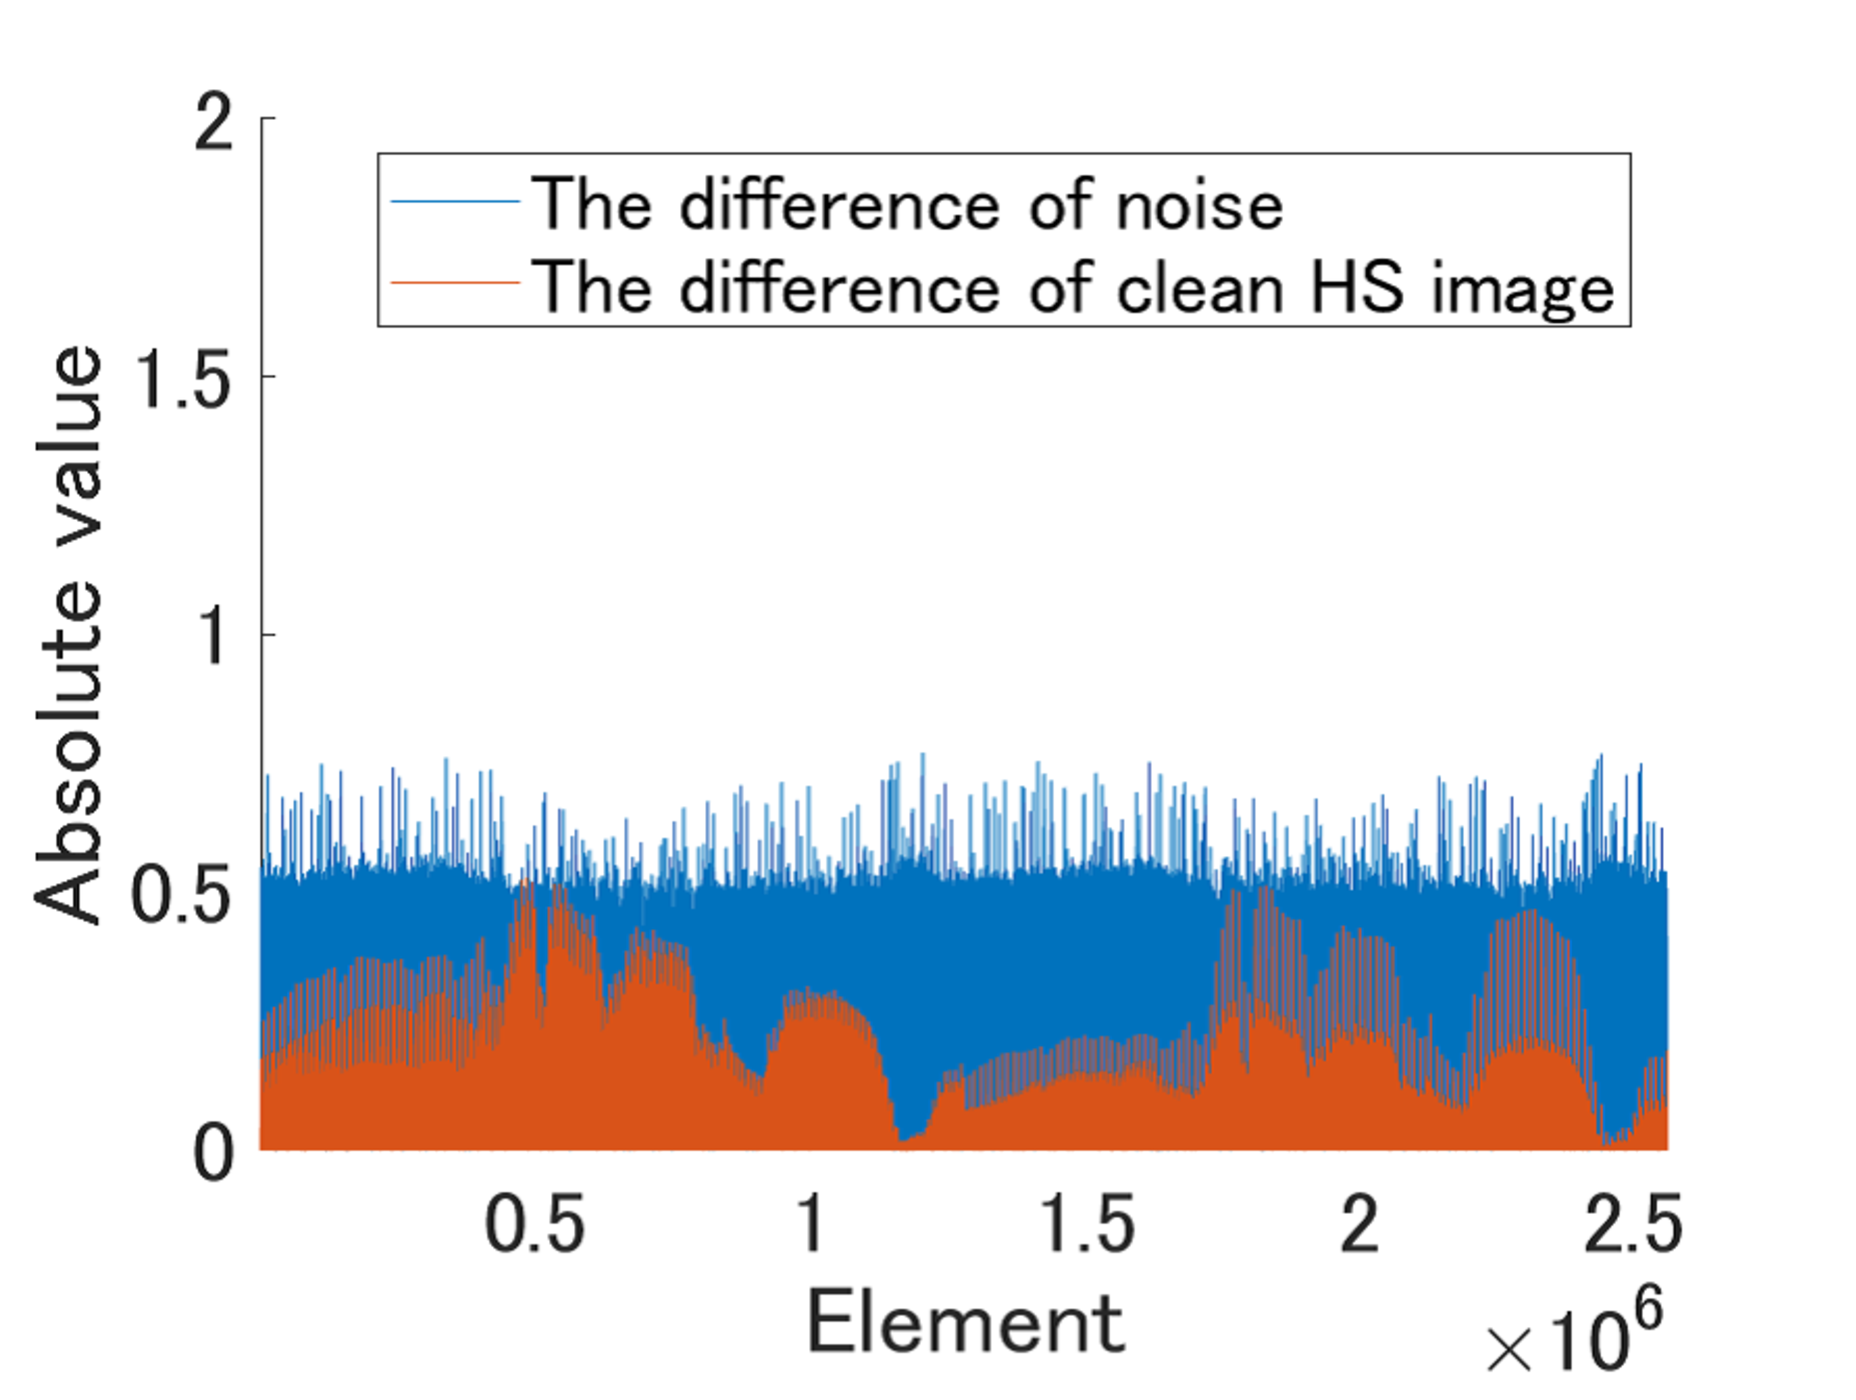
\includegraphics[width=\hsize]{./fig_supplement/compare_sparsity/Beltsville_first_order_differences.eps}}
		\end{minipage}
		
		\vspace{1mm}
		
		\makebox[0pt][r]{\raisebox{-6mm}{\rotatebox{90}{\shortstack{Second-order\\ differences}}} \hspace{2mm}}%
		\begin{minipage}{0.320\hsize}
			\centerline{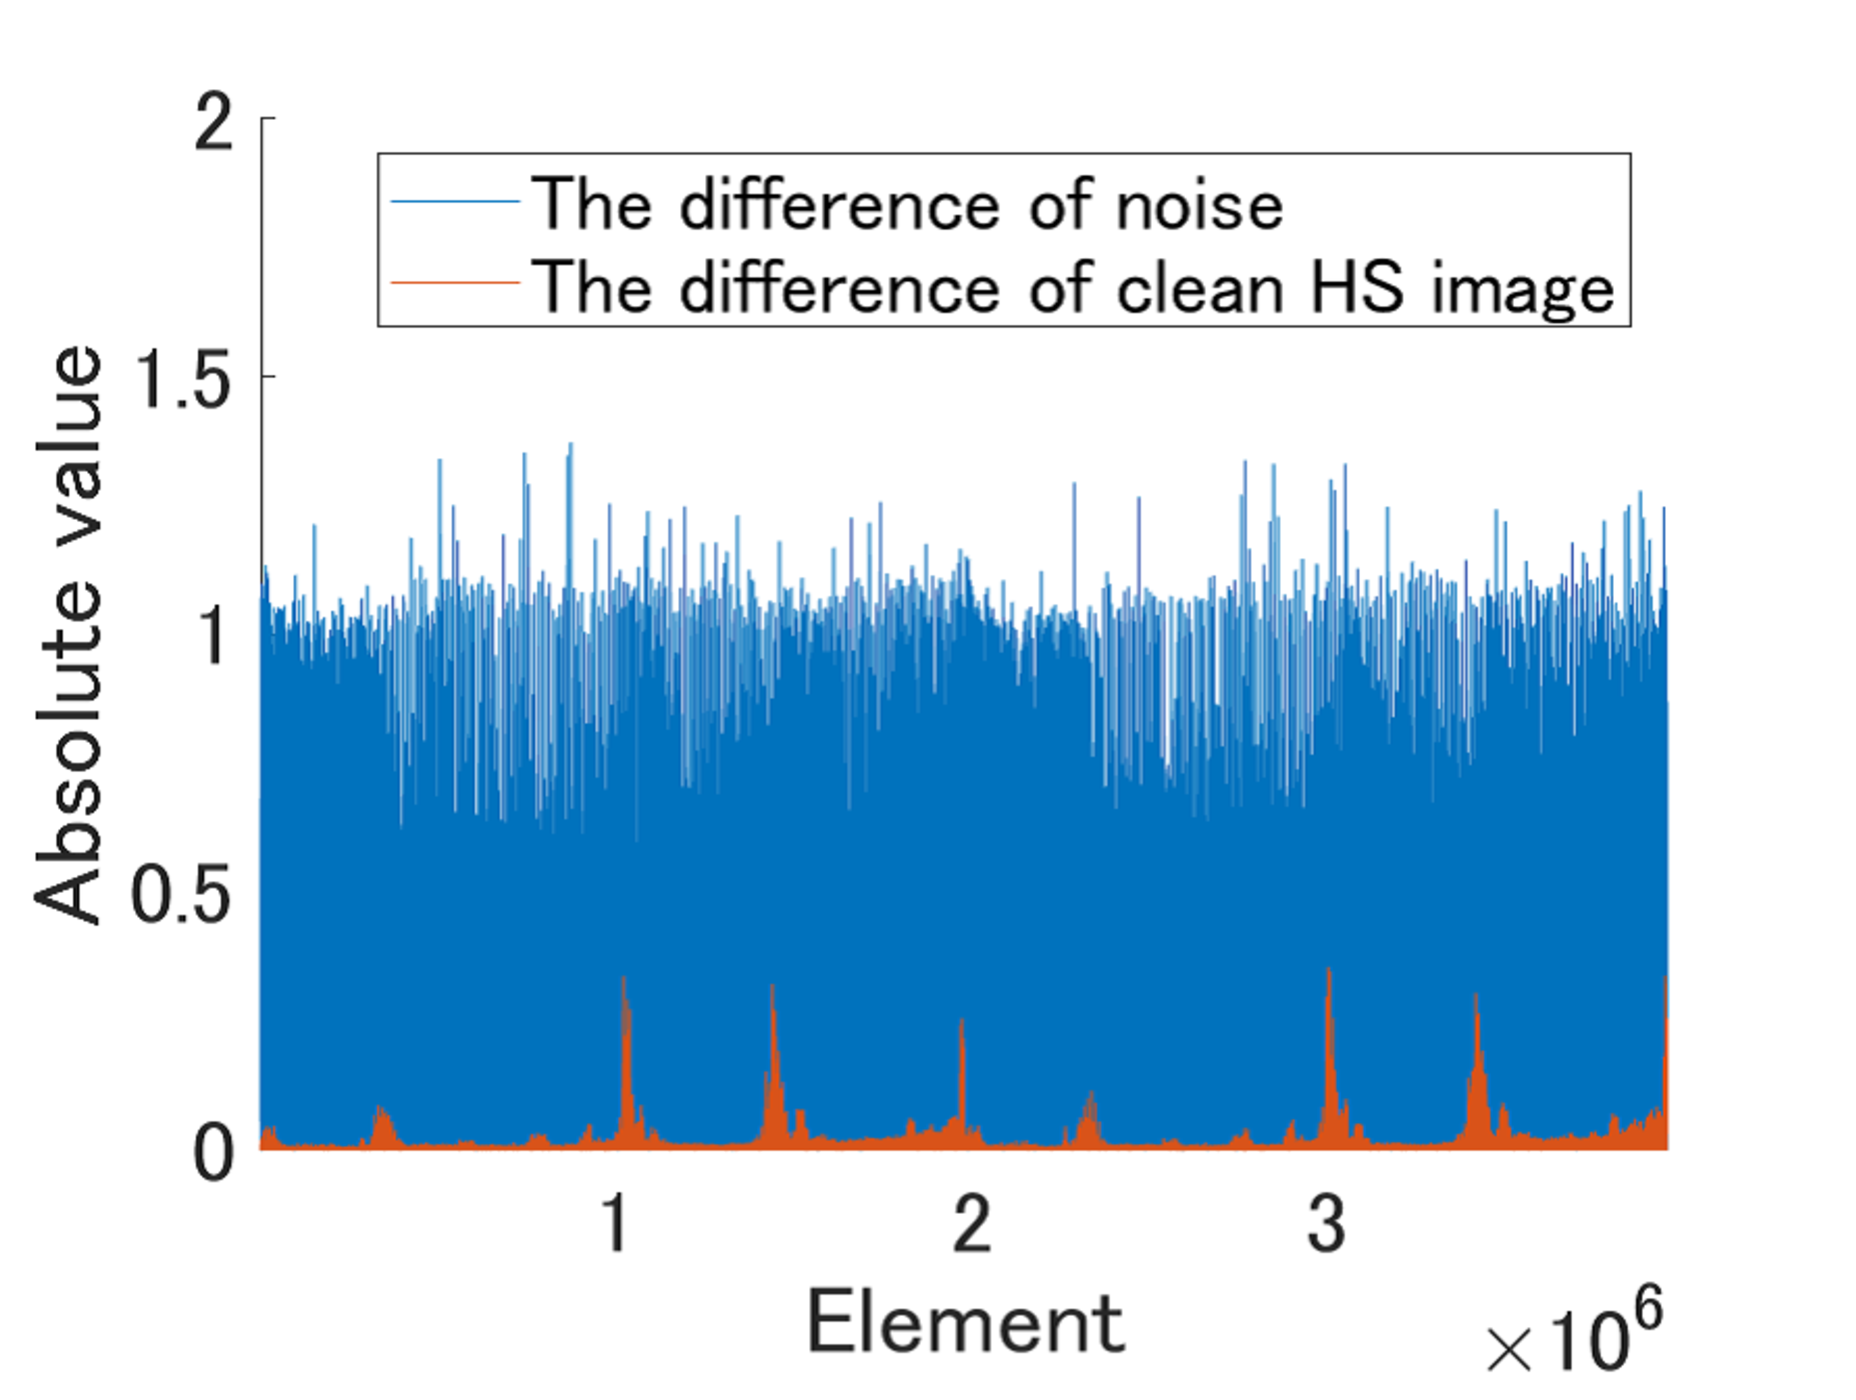
\includegraphics[width=\hsize]{./fig_supplement/compare_sparsity/JasperRidge_second_order_differences.eps}}
		\end{minipage}
		\begin{minipage}{0.320\hsize}
			\centerline{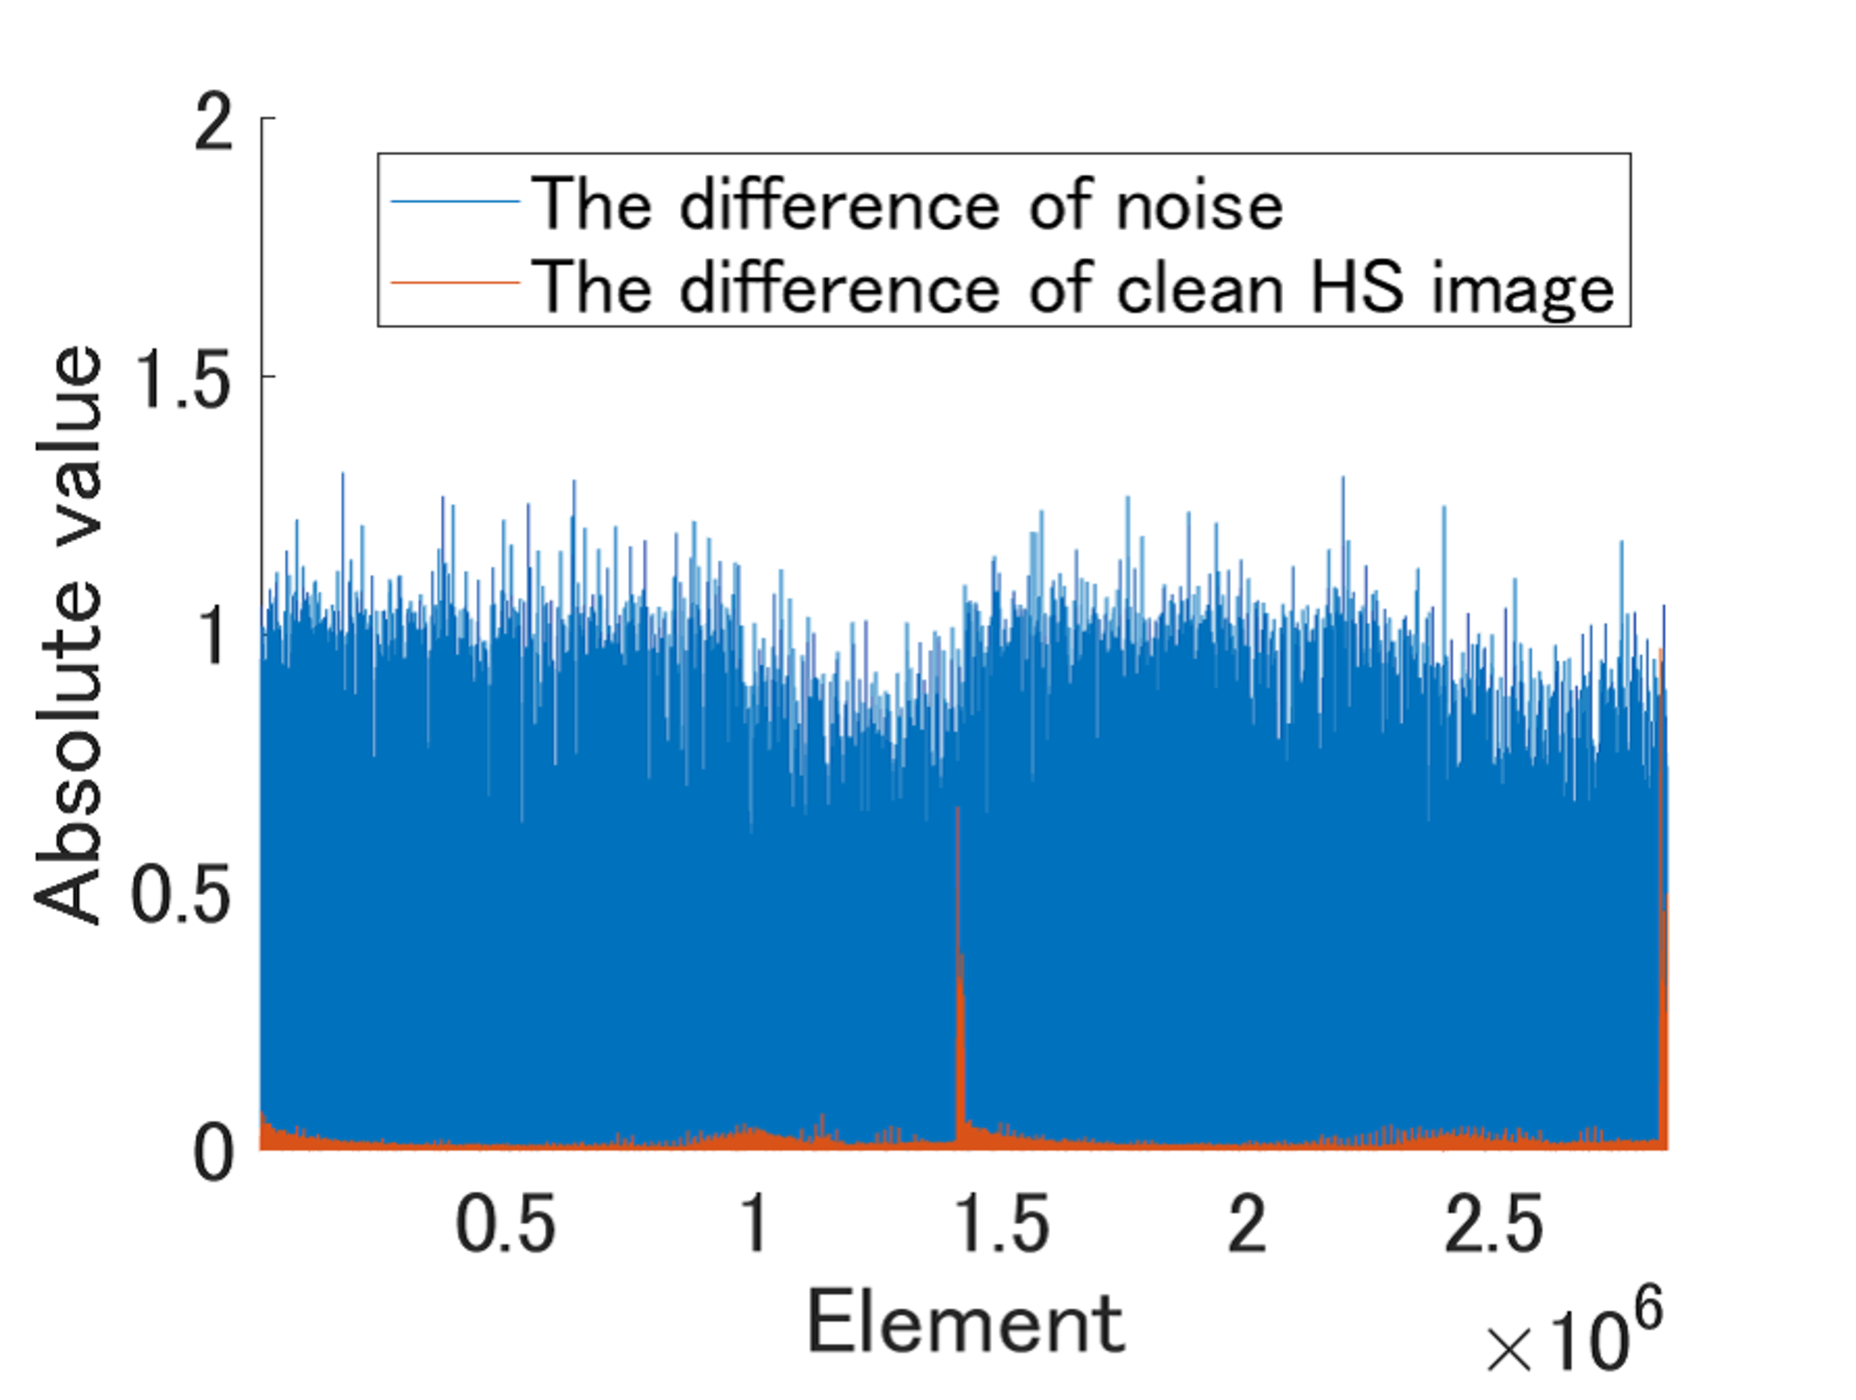
\includegraphics[width=\hsize]{./fig_supplement/compare_sparsity/PaviaU120_second_order_differences.eps}}
		\end{minipage}
		\begin{minipage}{0.320\hsize}
			\centerline{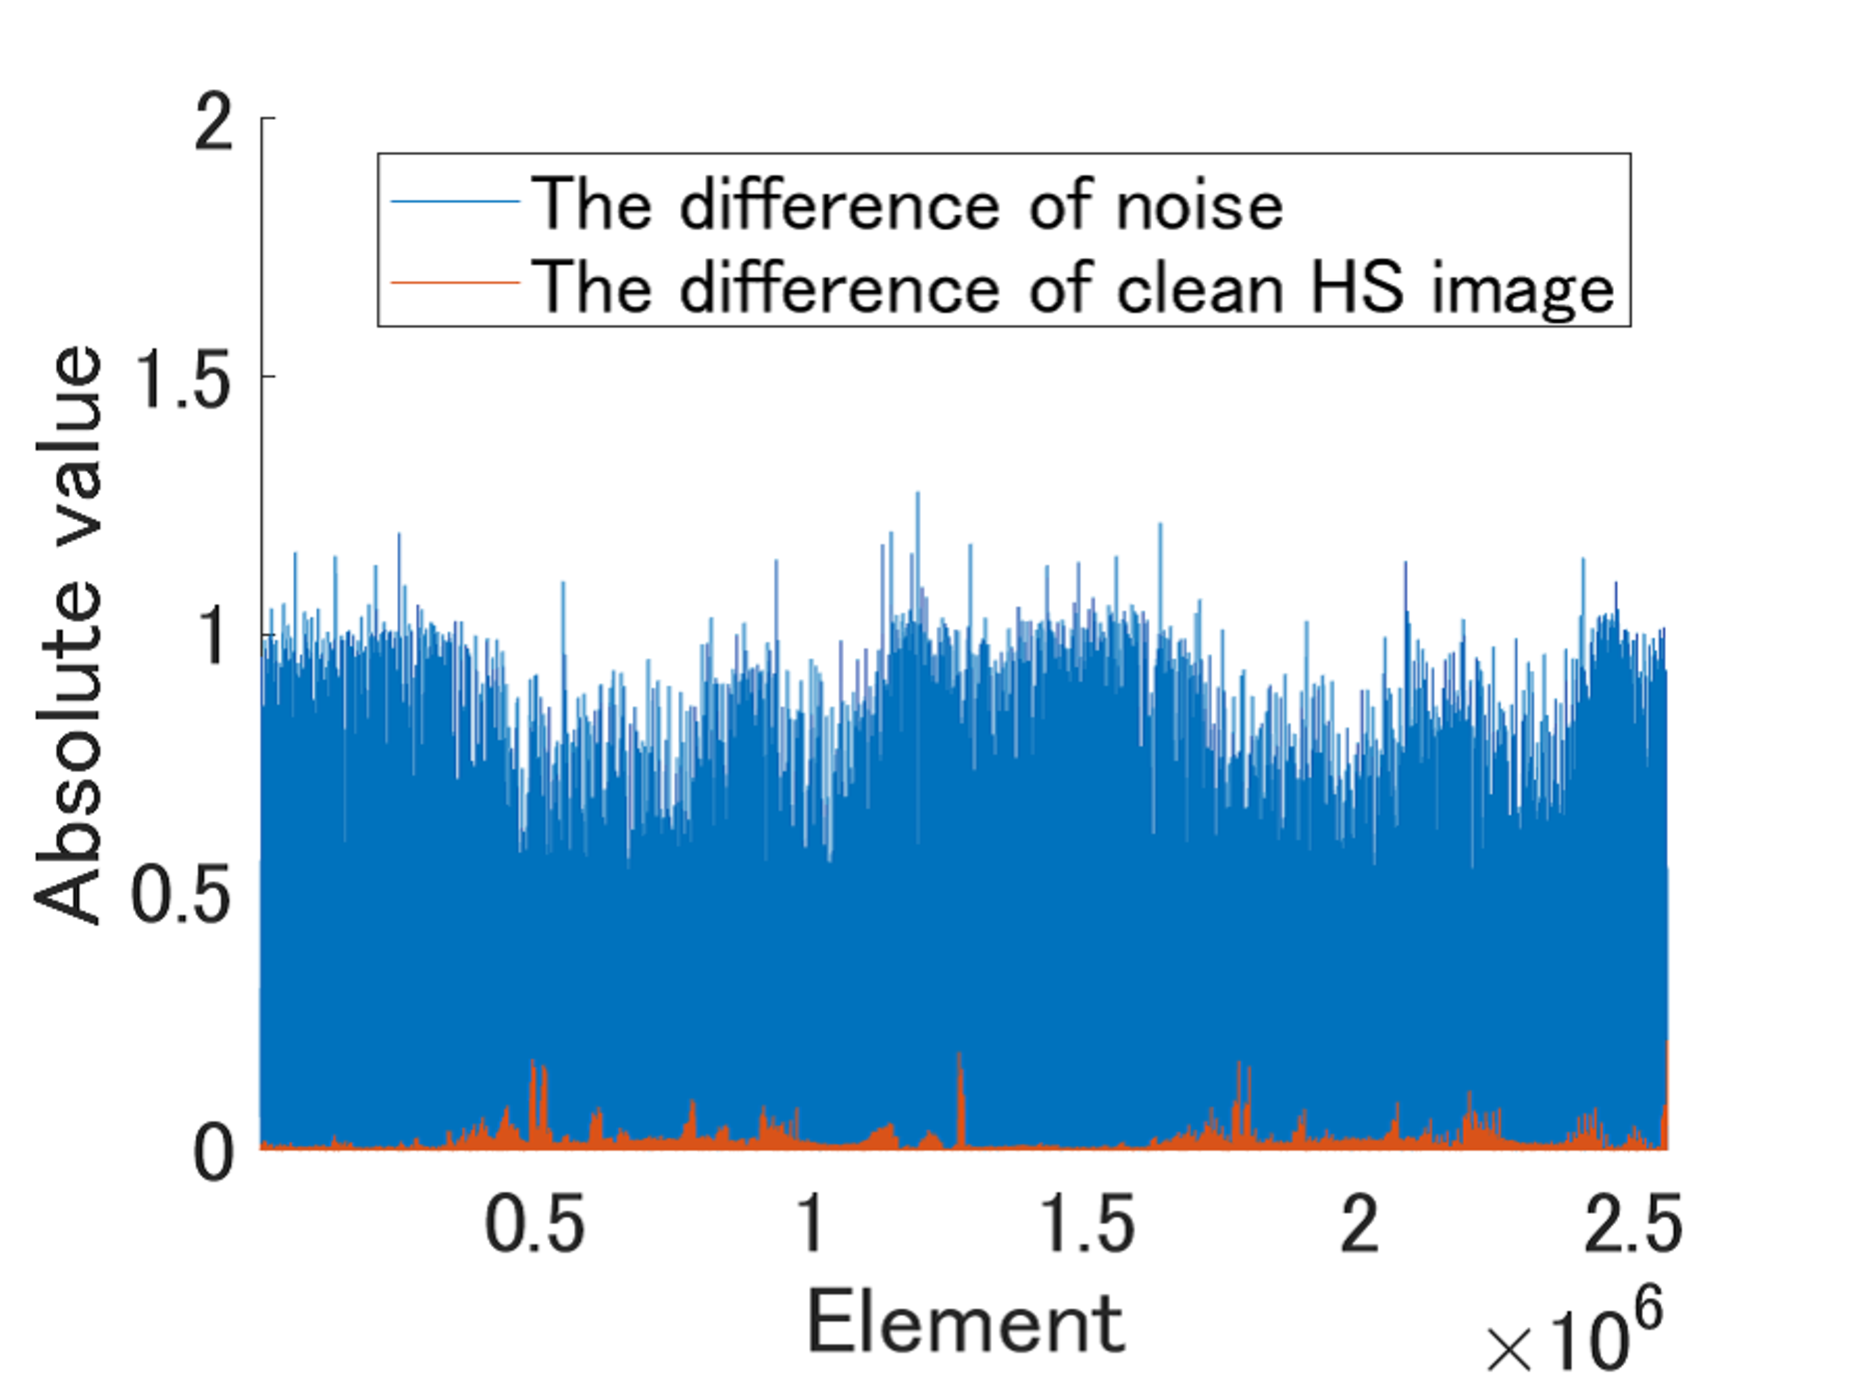
\includegraphics[width=\hsize]{./fig_supplement/compare_sparsity/Beltsville_second_order_differences.eps}}
		\end{minipage}
		
		\begin{minipage}{0.005\hsize}
			\centerline{\hspace{\hsize}} % Space
		\end{minipage}
		\begin{minipage}{0.320\hsize}
			\centerline{\small{(a)}}
		\end{minipage}
		\begin{minipage}{0.320\hsize}
			\centerline{\small{(b)}}
		\end{minipage}
		\begin{minipage}{0.320\hsize}
			\centerline{\small{(c)}}
		\end{minipage}
		
	\end{center}
	
	\caption{Absolute values of first-order and second-order differences in each image. (a): Jasper Ridge. (b): Pavia University. (c): Beltsville.}
	
	\label{fig:comparison_sparsity}
\end{figure*}